\section*{WRITING TASK 1}
You should spend about 20 minutes on this task.

\begin{quote}\large The line graph shows the average number of daily visits to three public libraries in the fictional city of Bellford between 2010 and 2025.
\end{quote}
Describe the main features of the information, select relevant details, and make comparisons where appropriate.

\begin{center}
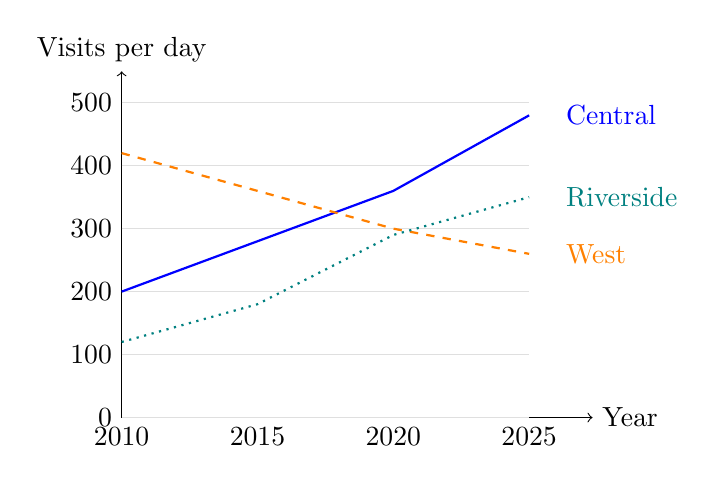
\begin{tikzpicture}[x=0.115cm,y=0.008cm]
\draw[->] (0,0)--(52,0) node[right]{Year}; \draw[->] (0,0)--(0,550) node[above]{Visits per day};
\foreach \v in {0,100,200,300,400,500}{\draw[gray!25] (0,\v)--(45,\v);\node[left] at (0,\v){\v};}
\foreach \x/\v in {0/2010,15/2015,30/2020,45/2025}{\node[below] at (\x,0){\v};}
\draw[blue,thick] (0,200)--(15,280)--(30,360)--(45,480);
\draw[orange,thick,dashed] (0,420)--(15,360)--(30,300)--(45,260);
\draw[teal,thick,dotted] (0,120)--(15,180)--(30,290)--(45,350);
\node[blue,anchor=west] at (48,480){Central};\node[orange,anchor=west] at (48,260){West};\node[teal,anchor=west] at (48,350){Riverside};
\end{tikzpicture}
\end{center}
Write at least 150 words.
\par\bigskip
{\footnotesize\color{gray} Original practice material; fictional settings and data. Not an official IELTS examination paper.}
